\documentclass[10pt,a4paper]{report}
\usepackage[utf8]{inputenc}
\usepackage{amsmath}
\usepackage{amsfonts}
\usepackage{amssymb}
\usepackage{amsthm}
\usepackage{hyperref}

\usepackage{multicol}
\usepackage{fancyhdr}
\usepackage{enumitem}
\usepackage{tikz}
\usepackage{tikz-cd}
\usetikzlibrary{calc}
\usetikzlibrary{shapes.geometric}
\usepackage[margin=0.5in]{geometry}
\usepackage{xcolor}
\DeclareMathOperator{\RANGE}{range}
\DeclareMathOperator{\NULL}{null}

\hypersetup{
    colorlinks=true,
    linkcolor=blue,
    filecolor=magenta,      
    urlcolor=cyan,
    pdftitle={Tensors},
    pdfpagemode=FullScreen,
    }

%\urlstyle{same}

\newcommand{\CLASSNAME}{Functional Analysis}
\newcommand{\STUDENTNAME}{Paul Carmody}
\newcommand{\ASSIGNMENT}{Assignment \#3}
\newcommand{\DUEDATE}{March 17, 2024}
\newcommand{\SEMESTER}{Spring 2024}
\newcommand{\SCHEDULE}{T/Th 9:30 -- 10:45}
\newcommand{\ROOM}{Remote}

\pagestyle{fancy}
\fancyhf{}
\chead{ \fancyplain{}{\CLASSNAME} }
%\chead{ \fancyplain{}{\STUDENTNAME} }
\rhead{\thepage}
\newcommand{\LET}{\text{Let }}
%\newcommand{\IF}{\text{if }}
\newcommand{\AND}{\text{ and }}
\newcommand{\OR}{\text{ or }}
\newcommand{\FORSOME}{\text{ for some }}
\newcommand{\FORALL}{\text{ for all }}
\newcommand{\WHERE}{\text{ where }}
\newcommand{\WTS}{\text{ WTS }}
\newcommand{\WLOG}{\text{ WLOG }}
\newcommand{\BS}{\backslash}
\newcommand{\DEFINE}[1]{\textbf{\emph{#1}}}
\newcommand{\IF}{$(\Rightarrow)$}
\newcommand{\ONLYIF}{$(\Leftarrow)$}
\newcommand{\ITH}{\textsuperscript{th} }
\newcommand{\FST}{\textsuperscript{st} }
\newcommand{\SND}{\textsuperscript{nd} }
\newcommand{\TRD}{\textsuperscript{rd} }
\newcommand{\INV}{\textsuperscript{-1} }

\newcommand{\XXX}{\mathfrak{X}}
\newcommand{\MMM}{\mathfrak{M}}
%\newcommand{\????}{\textfrak{A}}
%\newcommand{\????}{\textgoth{A}}
%\newcommand{\????}{\textswab{A}}

\DeclareMathOperator{\DER}{Der}
\DeclareMathOperator{\SGN}{sgn}

%%%%%%%
% derivatives
%%%%%%%

\newcommand{\PART}[2]{\frac{\partial #1}{\partial #2}}
\newcommand{\SPART}[2]{\frac{\partial^2 #1}{\partial #2^2}}
\newcommand{\DERIV}[2]{\frac{d #1}{d #2}}
\newcommand{\LAPLACIAN}[1]{\frac{\partial^2 #1}{\partial x^2} + \frac{\partial^2 #1}{\partial y^2}}

%%%%%%%
% sum, product, union, intersections
%%%%%%%

\newcommand{\SUM}[2]{\underset{#1}{\overset{#2}{\sum}}}
\newcommand{\PROD}[2]{\underset{#1}{\overset{#2}{\prod}}}
\newcommand{\UNION}[2]{\underset{#1}{\overset{#2}{\bigcup}}}
\newcommand{\INTERSECT}[2]{\underset{#1}{\overset{#2}{\bigcap}}}
\newcommand{\FSUM}{\SUM{n=-\infty}{\infty}}
       

%%%%%%%
% supremum and infimum
%%%%%%%

\newcommand{\SUP}[1]{\underset{#1}\sup \,}
\newcommand{\INF}[1]{\underset{#1}\inf \,}
\newcommand{\MAX}[1]{\underset{#1}\max \,}
\newcommand{\MIN}[1]{\underset{#1}\min \,}

%%%%%%%
% infinite sums, limits
%%%%%%%

\newcommand{\SUMK}{\SUM{k=1}{\infty}}
\newcommand{\SUMN}{\SUM{n=1}{\infty}}
\newcommand{\SUMKZ}{\SUM{k=0}{\infty}}
\newcommand{\LIM}[1]{\underset{#1}\lim\,}
\newcommand{\IWOB}[1]{\LIM{#1 \to \infty}}
\newcommand{\LIMK}{\IWOB{k}}
\newcommand{\LIMN}{\IWOB{n}}
\newcommand{\LIMX}{\IWOB{x}}
\newcommand{\NIWOB}{\LIM{n \to \infty}}
\newcommand{\LIMSUPK}{\underset{k\to\infty}\limsup \,}
\newcommand{\LIMSUPN}{\underset{n\to\infty}\limsup \,}
\newcommand{\LIMINFK}{\underset{k\to\infty}\liminf \,}
\newcommand{\LIMINFN}{\underset{n\to\infty}\liminf \,}
\newcommand{\ROOTRULE}[1]{\LIMSUPK \BARS{#1}^{1/k}}

\newcommand{\CUPK}{\bigcup_{k=1}^{\infty}}
\newcommand{\CAPK}{\bigcap_{k=1}^{\infty}}
\newcommand{\CUPN}{\bigcup_{n=1}^{\infty}}
\newcommand{\CAPN}{\bigcap_{n=1}^{\infty}}

%%%%%%%
% number systems (real, rational, etc.)
%%%%%%%

\newcommand{\REALS}{\mathbb{R}}
\newcommand{\RATIONALS}{\mathbb{Q}}
\newcommand{\IRRATIONALS}{\REALS \backslash \RATIONALS}
\newcommand{\INTEGERS}{\mathbb{Z}}
\newcommand{\NUMBERS}{\mathbb{N}}
\newcommand{\COMPLEX}{\mathbb{C}}
\newcommand{\DISC}{\mathbb{D}}
\newcommand{\HPLANE}{\mathbb{H}}

\newcommand{\R}{\mathbb{R}}
\newcommand{\Q}{\mathbb{Q}}
\newcommand{\Z}{\mathbb{Z}}
\newcommand{\N}{\mathbb{N}}
\newcommand{\C}{\mathbb{C}}
\newcommand{\T}{\mathbb{T}}
\newcommand{\COUNTABLE}{\aleph_0}
\newcommand{\UNCOUNTABLE}{\aleph_1}


%%%%%%%
% Arithmetic/Algebraic operators
%%%%%%%


\DeclareMathOperator{\MOD}{mod}
%\newcommand{\MOD}[1]{\mod #1}
\newcommand{\BAR}[1]{\overline{#1}}
\newcommand{\LCM}{\text{ lcm}}
\newcommand{\ZMOD}[1]{\Z/#1\Z}
\DeclareMathOperator{\VAR}{Var}
%%%%%%%
% complex operators
%%%%%%%

\DeclareMathOperator{\RR}{Re}
%\newcommand{\RE}{\text{Re}}
\DeclareMathOperator{\IM}{Im}
%\newcommand{\IM}{\text{Im}}
\newcommand{\CONJ}[1]{\overline{#1}}
\DeclareMathOperator{\LOG}{Log}
%\newcommand{\LOG}{\text{ Log }}
\newcommand{\RES}[2]{\underset{#1}{\text{res}} #2}

%%%%%%%
% Group operators
%%%%%%%

\newcommand{\AUT}{\text{Aut}\,}
\newcommand{\KER}{\text{ker}\,}
\newcommand{\END}{\text{End}}
\newcommand{\HOM}{\text{Hom}}
\newcommand{\CYCLE}[1]{(\begin{array}{cccccccccc}
		#1
	\end{array})}
\newcommand{\SUBGROUP}{\underset{\text{group}}\subseteq}	
%\newcommand{\SUBGROUP}{\subseteq_g}
\newcommand{\SUBRING}{\underset{\text{ring}}\subseteq}
\newcommand{\SUBMOD}{\underset{\text{mod}}\subseteq}
\newcommand{\SUBFIELD}{\underset{\text{field}}\subseteq}
\newcommand{\ISO}{\underset{\text{iso}}\longrightarrow}
\newcommand{\HOMO}{\underset{\text{homo}}\longrightarrow}

%%%%%%%
% grouping (parenthesis, absolute value, square, multi-level brackets).
%%%%%%%

\newcommand{\PAREN}[1]{\left (\, #1 \,\right )}
\newcommand{\BRACKET}[1]{\left \{\, #1 \,\right \}}
\newcommand{\SQBRACKET}[1]{\left [\, #1 \,\right ]}
\newcommand{\ABRACKET}[1]{\left \langle\, #1 \,\right \rangle}
\newcommand{\BARS}[1]{\left |\, #1 \,\right |}
\newcommand{\DBARS}[1]{\left \| \, #1 \,\right \|}
\newcommand{\LBRACKET}[1]{\left \{ #1 \right .} 
\newcommand{\RBRACKET}[1]{\left . #1 \right \]}
\newcommand{\RBAR}[1]{\left . #1 \, \right |}
\newcommand{\LBAR}[1]{\left | \, #1 \right .}
\newcommand{\BLBRACKET}[2]{\BRACKET{\RBAR{#1}#2}}
\newcommand{\GEN}[1]{\ABRACKET{#1}}
\newcommand{\BINDEF}[2]{\LBRACKET{\begin{array}{ll}
     #1\\
     #2
\end{array}}}

%%%%%%%
% Fourier Analysis
%%%%%%%

\newcommand{\ONEOTWOPI}{\frac{1}{2\pi}}
\newcommand{\FHAT}{\hat{f}(n)}
\newcommand{\FINT}{\int_{-\pi}^\pi}
\newcommand{\FINTWO}{\int_{0}^{2\pi}}
\newcommand{\FSUMN}[1]{\SUM{n=-#1}{#1}}
%\newcommand{\FSUM}{\SUMN{\infty}}
\newcommand{\EIN}[1]{e^{in#1}}
\newcommand{\NEIN}[1]{e^{-in#1}}
\newcommand{\INTALL}{\int_{-\infty}^{\infty}}
\newcommand{\FTINT}[1]{\INTALL #1 e^{2\pi inx\xi} dx}
\newcommand{\GAUSS}{e^{-\pi x^2}}

%%%%%%%
% formatting 
%%%%%%%

\newcommand{\LEFTBOLD}[1]{\noindent\textbf{#1}}
\newcommand{\SEQ}[1]{\{#1\,\}}
\newcommand{\WIP}{\footnote{work in progress}}
\newcommand{\QED}{\hfill\square}
\newcommand{\ts}{\textsuperscript}
\newcommand{\HLINE}{\noindent\rule{7in}{1pt}\\}

%%%%%%%
% Mathematical note taking (definitions, theorems, etc.)
%%%%%%%

\newcommand{\REM}{\noindent\textbf{\\Remark: }}
\newcommand{\DEF}{\noindent\textbf{\\Definition: }}
\newcommand{\THE}{\noindent\textbf{\\Theorem: }}
\newcommand{\COR}{\noindent\textbf{\\Corollary: }}
\newcommand{\LEM}{\noindent\textbf{\\Lemma: }}
\newcommand{\PROP}{\noindent\textbf{\\Proposition: }}
\newcommand{\PROOF}{\noindent\textbf{\\Proof: }}
\newcommand{\EXP}{\noindent\textbf{\\Example: }}
\newcommand{\TRICKS}{\noindent\textbf{\\Tricks: }}


%%%%%%%
% text highlighting
%%%%%%%

\newcommand{\B}[1]{\textbf{#1}}
\newcommand{\CAL}[1]{\mathcal{#1}}
\newcommand{\UL}[1]{\underline{#1}}

%%%%%%
% Linear Algebra
%%%%%%

\newcommand{\COLVECTOR}[1]{\PAREN{\begin{array}{c}
#1
\end{array} }}
\newcommand{\TWOXTWO}[4]{\PAREN{ \begin{array}{c c} #1&#2 \\ #3 & #4 \end{array} }}
\newcommand{\DTWOXTWO}[4]{\BARS{ \begin{array}{c c} #1&#2 \\ #3 & #4 \end{array} }}
\newcommand{\THREEXTHREE}[9]{\PAREN{ \begin{array}{c c c} #1&#2&#3 \\ #4 & #5 & #6 \\ #7 & #8 & #9 \end{array} }}
\newcommand{\DTHREEXTHREE}[9]{\BARS{ \begin{array}{c c c} #1&#2&#3 \\ #4 & #5 & #6 \\ #7 & #8 & #9 \end{array} }}
\newcommand{\NXN}{\PAREN{ \begin{array}{c c c c} 
			a_{11} & a_{12} & \cdots & a_{1n} \\
			a_{21} & a_{22} & \cdots & a_{2n} \\
			\vdots & \vdots & \ddots & a_{1n} \\
			a_{n1} & a_{n2} & \cdots & a_{nn} \\
		\end{array} }}
\newcommand{\SLR}{SL_2(\R)}
\newcommand{\GLR}{GL_2(\R)}
\DeclareMathOperator{\TR}{tr}
\DeclareMathOperator{\BIL}{Bil}
\DeclareMathOperator{\SPAN}{span}

%%%%%%%
%  White space
%%%%%%%

\newcommand{\BOXIT}[1]{\noindent\fbox{\parbox{\textwidth}{#1}}}


\newtheorem{theorem}{Theorem}[section]
\newtheorem{corollary}{Corollary}[theorem]
\newtheorem{lemma}[theorem]{Lemma}

\theoremstyle{definition}
\newtheorem{definition}[theorem]{Definition}
\newtheorem{prop}[theorem]{Proposition}

\theoremstyle{remark}
\newtheorem{remark}[theorem]{Remark}
\newtheorem{example}[theorem]{Example}
%\newtheorem*{proof}[theorem]{Proof}



\newcommand{\RED}[1]{\textcolor{red}{#1}}
\newcommand{\BLUE}[1]{\textcolor{blue}{#1}}
\newcommand{\GREEN}[1]{\textcolor{black!30!green}{#1}}
\newcommand{\ORANGE}[1]{\textcolor{orange}{#1}}
\newcommand{\F}{\textbf{F}}

\title{Advanced Linear Algebra}
\author{The Unforgetable Someone}
\date{Summer 2023}

\newcommand{\NORM}[1]{\,\left \Vert #1 \right \Vert}
\begin{document}

\begin{center}
	\Large{\CLASSNAME -- \SEMESTER} \\
\end{center}
\begin{center}
	\STUDENTNAME \\
	\ASSIGNMENT -- \DUEDATE\\
\end{center} 
p. 126 \#8 
Show that the dual space of the space $c_0$ is $\ell^1$.(Cf. Prob. 1 in Sec. 2.3.)\\
\\
Want to show that
\begin{enumerate}
	\item every element of $c_0'$ is an element of $\ell^1$
	
	Let $(e_k)$ be the unique Shauder basis for $\ell^1$ where $e_k = (\delta_{jk})$.  Let $x = (\xi_j) \in c_0$, that is $\LIM{j\to \infty} \xi_j = 0$ which has the unique representation $x=\SUM{j=1}{\infty} \xi_j e_j$. Let $f \in c_0'$, that is $f: c_0 \to \R$ which is linear and bounded.  Therefore, 
	\begin{align*}
		f(x) &= \SUM{j=1}{\infty} \xi_j f(e_j)\\
		|f(e_j)| &\le \NORM{f}\NORM{e_j} = \NORM{f} \\
		\NORM{f(x)} &\le \NORM{f} \BARS{\SUM{j=1}{\infty} \xi_j} \le \NORM{f} \SUM{j=1}{\infty} |\xi_j| = \NORM{f} \NORM{x}_{\ell^1}
	\end{align*}which means that $f \in \ell^1$.
	
	\item that the norm over $c_0'$ is the norm over $\ell^1$.  want to show that $|f(x)| = \NORM{x}$.  Let $\gamma = \SUP{j} f(e_j)$
	\begin{align*}
		|f(x)| &= \BARS{\SUM{j=1}{\infty} \xi_j f(e_j)} \le \gamma \SUM{j=1}{\infty} |\xi_j| = \gamma \NORM{x}
	\end{align*}
\end{enumerate}


\noindent p. 135 \#9 Prove
\begin{align*}
	\RR \ABRACKET{x,y} &= \frac{1}{4}\PAREN{\NORM{x+y}^2-\NORM{x-y}^2} \\
	\IM \ABRACKET{x,y} &= \frac{1}{4}\PAREN{\NORM{x+iy}^2-\NORM{x-iy}^2} 
\end{align*} Remember that
\begin{align*}
	\NORM{x+y}^2 &= \NORM{x}^y + \NORM{y}^2 +2 \RR \ABRACKET{x,y}\\
	\text{ and } \NORM{x+y}^2+\NORM{x-y}^2 &= 2 \NORM{x}^2+2\NORM{y}^2 \\
	\text{ thus } 2 \RR \ABRACKET{x,y} &= \NORM{x+y}^2 - \NORM{x}^2 - \NORM{y}^2 \\
	&= \NORM{x+y}^2 - (\NORM{x}^2 + \NORM{y}^2) \\
	&= \NORM{x+y}^2 - \frac{1}{2}\PAREN{ \NORM{x+y}^2+\NORM{x-y}^2} \\
	4 \RR \ABRACKET{x,y} &= \NORM{x+y}^2-\NORM{x-y}^2 \\
	\RR \ABRACKET{x,y} &= \frac{1}{4}\PAREN{\NORM{x+y}^2-\NORM{x-y}^2} \\
\end{align*}Notice that 
\begin{align*}
	\text{ Notice } \NORM{x+iy}^2+\NORM{x-iy}^2 &= 2 \NORM{x}^2+2\NORM{y}^2\\
	\NORM{x-iy}^2 &= \ABRACKET{x-iy,x-iy}\\
		&= \ABRACKET{x,x-iy}+\ABRACKET{iy,x-iy} \\
		&= \ABRACKET{x,x} + \ABRACKET{x,iy} -\ABRACKET{iy,x}+\ABRACKET{iy,iy}\\
		&= \NORM{x}^2 + |i|^2\NORM{y}^2 -i\ABRACKET{x,y} -i\CONJ{\ABRACKET{x,y}} \\
		&= \NORM{x}^2 + \NORM{y}^2 + 2\IM\ABRACKET{x,y} \\
	2\IM\ABRACKET{x,y} &= \NORM{x-iy}^2 - \PAREN{\NORM{x}^2 + \NORM{y}^2} \\
		&= \NORM{x-iy}^2 - \frac{1}{2}\PAREN{\NORM{x+iy}^2+\NORM{x-iy}^2} \\
	4\IM\ABRACKET{x,y} &= \NORM{x-iy}^2 -\NORM{x+iy}^2\\
\end{align*}

\newpage
p. 141 \#7-10, 
\begin{enumerate}
	\setcounter{enumi}{6}
	\item Show that in an inner product space, $x \perp y$ if and only if $\NORM{x+\alpha y}=\NORM{x-\alpha y}$ (see Fig. 25.)\\
	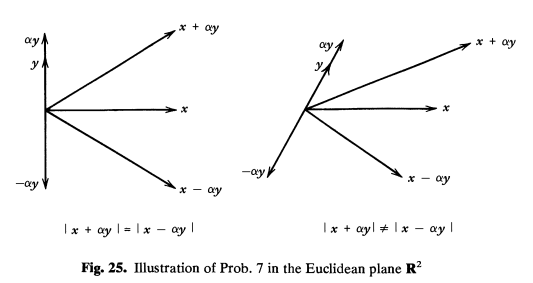
\includegraphics[scale=0.8]{711_03_fig25.png} \\
	Assuming that $x \perp y$ then $\ABRACKET{x,y} = 0$ and
	\begin{align*}
		\NORM{x+\alpha y}^2 &= \NORM{x}^2 + |\alpha|^2\NORM{y}^2 +2|\alpha|\RR\ABRACKET{x,y} \\
		&= \NORM{x}^2 + |\alpha|^2\NORM{y}^2 \\
		\NORM{x-\alpha y}^2 &= \NORM{x}^2 + |\alpha|^2\NORM{y}^2 -2|\alpha|\RR\ABRACKET{x,y} \\
		&= \NORM{x}^2 + |\alpha|^2\NORM{y}^2
	\end{align*}Asuming that they are equal
	\begin{align*}
		\NORM{x+\alpha y}^2-\NORM{x-\alpha y}^2 &= \PAREN{\NORM{x}^2 + |\alpha|^2\NORM{y}^2 +2|\alpha|\RR\ABRACKET{x,y}} - \PAREN{\NORM{x}^2 + |\alpha|^2\NORM{y}^2 -2\BARS{\alpha}\RR\ABRACKET{x,y}} \\
		&= 4|\alpha|\RR\ABRACKET{x,y}
	\end{align*}which can  only be zero when $\RR\ABRACKET{x,y}=0$ or $x \perp y$.
	
	\item Show that in an inner product space, $x \perp y$ if and only if $\NORM{x+\alpha y}\ge \NORM{x}$ for all scalars $\alpha$.\\
	
	Assuming that $x \perp y$ then
	\begin{align*}
		\NORM{x+\alpha y}^2 &= \NORM{x}^2 + |\alpha|^2\NORM{y}^2 +2|\alpha|\RR\ABRACKET{x,y} \\
		&= \NORM{x}^2 + |\alpha|^2\NORM{y}^2
	\end{align*}$|\alpha| \ge 0$ for all $\alpha$ as well as $\NORM{y} \ge 0$ for all $y$.  Thus, $\NORM{x+\alpha y}\ge \NORM{x}$.\\
	Assuming that this statement is true then for all $\alpha \in \C$ and $y \in Y$
	\begin{align*}
		\NORM{x}^2 + |\alpha|^2\NORM{y}^2 +2|\alpha|\RR\ABRACKET{x,y} &\ge \NORM{x}^2 \\
		|\alpha|^2\NORM{y}^2 +2|\alpha|\RR\ABRACKET{x,y} &\ge 0 \\
		|\alpha|^2\NORM{y}^2 &\ge -2|\alpha|\RR\ABRACKET{x,y}
	\end{align*}the left side is positive and the right side is negative therefore $\RR\ABRACKET{x,y}=0$ and $x \perp y$.
	
	\newpage
	\item Let $V$ be the vector space of all continuous complex-valued functions on $J=[a,b]$.  Let $X_1 = \PAREN{V, \NORM{\cdot}_\infty}$, where $\NORM{x}_\infty = \MAX{t\in J}\BARS{x(t)}$; and let $X_2 = \PAREN{V, \NORM{\cdot}_2}$, where
	\begin{align*}
		\NORM{x}_2 = \ABRACKET{x,x}^{1/2}, \text{     } \ABRACKET{x,y} = \int_a^b x(t)\CONJ{y(t)} dt
	\end{align*}  Show that the identity mapping $x \mapsto x$ of $X_1$ onto $X_2$ is continuous.\\(It is not a homeomorphism.  $X_2$ is not complete.)\\
	
	Let $T: X_1 \to X_2$ such that $Tx=x$.  We want to show that given any $\epsilon > 0$ when $\NORM{Tx - Ty} < \epsilon$, then $\NORM{x-y} \le \delta$ for some $\delta>0$ dependent on $\epsilon$.
	\begin{align*}
		\epsilon > \NORM{Tx - Ty}_2^2 &= \ABRACKET{x-y, x-y} \\
		&= \int_a^b \PAREN{x(t)-y(t)}\CONJ{\PAREN{x(t)-y(t)}}dt \\
		&= \int_a^b \RR\PAREN{x(t)-y(t)}^2 + \IM\PAREN{x(t)-y(t)}^2 dt \\
		&\ge \int_a^b \NORM{x(t)-y(t)}_2^2 dt
	\end{align*}by the Extreme Value Theorem, there exists $p \in J$ such that $x(p) \ge x(t)-y(t),\forall t\in J$ i.e., $|x(p)-y(p)| = \NORM{x-y}_\infty$.  Thus.
	\begin{align*}
		\int_a^b \NORM{x(t)-y(t)}_2^2 dt \le (b-a) (x(p)-y(p))^2 = (b-a)\NORM{x-y}_\infty^2 < \delta
	\end{align*}
	
	\item \textbf{(Zero Operator)}  Let $T: X \to X$ be a bounded linear operator on a complex inner product space $X$.  If $\ABRACKET{Tx,x} = 0$ for all $x \in X$, show that $T=0$.\\
	Show that this does not hold in the case of a real inner product space. \textit{Hint.} Consider a rotation of the Euclidiean plane.
	\begin{align*}
		0 &= \ABRACKET{T(x+y),x+y} \\
		&= \ABRACKET{Tx+Ty, x+y} \\
		&= \ABRACKET{Tx, x+y}+\ABRACKET{Ty,x+y} \\
		&= \ABRACKET{Tx,x} + \ABRACKET{Tx,y} + \ABRACKET{Ty,x} + \ABRACKET{Ty,y}\\
		&= \ABRACKET{Tx,y} + \ABRACKET{Ty,x}
	\end{align*}The Inner Product is positive definite, which means that the only way that the right side can be equal to zero is if $Tx=0$ for $x\in x$.
\end{enumerate}
\newpage
p. 150 \#2, 3a, 6, 
\begin{enumerate}
	\setcounter{enumi}{1}
	\item Show that the subset $M = \{y =(\eta_j)\,|\, \sum \eta_j = 1\}$ of complex space $\textbf{C}^n$ (cf 3.1-4) is complete and convex.  Find the vector of minimum norm in $M$.
	
	\begin{align*}
		\ABRACKET{x,y} &= \sum \xi_j \CONJ{\eta_j}\\
		\NORM{x}^2 &= \sum \xi_j \CONJ{\xi_j}
	\end{align*}
	
	\item (a) Show that the vector space $X$ of all real-valued continuous functions on $[-1,1]$ is the direct sum of the set of all even continuous functions and the set of all odd continuous functions on $[-1,1]$.\\
	
	Define the inner product over the set of continuous functions on $[-1,1]$ as 
	\begin{align*}
		\ABRACKET{x,y} &= \int_{-1}^1 x(t)y(t) dt 
	\end{align*}Let $E$ be the set of even functions.  That is for all $f \in E$ then $f(x) = f(-x)$. Let $g \in E^\perp$ then
	\begin{align*}
		0 &= \ABRACKET{f,g} = \int_{-1}^1 f(t)g(t) dt\\
		&= \int_{-1}^0 f(t) g(t) dt + \int_{0}^1 f(t)g(t) dt\\
	\end{align*}notice that the function $h(t)=f(t)g(t)$ on $t\in[-1,1]$ is odd.  Yet, $f$ is even, thus $g$ must be odd.  Since $g$ is arbitrary $E^\perp$ is filled with odd functions. And we know that $X = E \oplus E^\perp$.
	
	\setcounter{enumi}{5}
	\item Show that $Y=\{x\,|\, x=(\xi_j)\in \ell^2, \xi_{2n}=0, n\in \N\}$ is a closed subspace of $\ell^2$ and find $Y^\perp$.  What is $Y^\perp$ if $Y=$ span$\{e_1,\cdots,e_n\}\subset \ell^2$, where $e_j = (\delta_{jk})$?\\
	\\
	Let $x = (\xi_j), y = (\eta_j) \in Y$.  Then, $x+\alpha y = (\xi_j + \alpha \eta_j)$.  Whenever, $j$ is even $\xi_j = \eta_j=0$ and $\xi_j + \alpha \eta_j = 0$ thus $x+\alpha y \in Y$. Further, let $x_n = (\xi^n_j) \in Y$ be a convergent sequence and $x_n \to x$.  NOTE: $\xi^n$ is NOT an exponent but an index.  Then
	\begin{align*}
		\NORM{x_n-x}^2 &= \sum_{i=1}^\infty (\xi^n_i-\xi_i)^2
	\end{align*}when $i$ is even we have zero.  Each of the terms on the right must be positive.  Thus, $\LIM{n \to \infty} \NORM{x_n -x}^2 = 0$ which implies that $\xi^m_n \to \xi_i$ for all $i\in \N$. Thus, $x \in Y$ and $Y$ is closed.\\
	\\
	

\end{enumerate}
\end{document}